\documentclass[11pt,a4paper]{article}
\usepackage[margin=2.2cm,top=2.6cm,bottom=2.2cm]{geometry}
% ===================== CONCLAVE Guide - shared preamble =====================
\usepackage[T1]{fontenc}
\usepackage[utf8]{inputenc}
\usepackage{lmodern}
\usepackage[scaled=0.92]{helvet}
\usepackage{courier}
\usepackage{amsmath,amssymb,amsthm}
\usepackage[table,dvipsnames]{xcolor}
\usepackage{graphicx}
\usepackage{booktabs}
\usepackage{array}
\usepackage{longtable}
\usepackage{enumitem}
\usepackage{tikz}
\usepackage{pgfplots}
\usepackage[most]{tcolorbox}
\usepackage{listings}
\usepackage{titlesec}
\usepackage{fancyhdr}
\usepackage{tocloft}
\usepackage[hidelinks]{hyperref}
\usetikzlibrary{positioning,arrows.meta,shapes.geometric,calc,fit,backgrounds,decorations.pathreplacing}
\pgfplotsset{compat=1.16}

% ------------------------------- palette --------------------------------
\definecolor{conclaveblue}   {HTML}{1B4F72}
\definecolor{conclavelight}  {HTML}{1B6CA8}
\definecolor{conclavesky}    {HTML}{5DADE2}
\definecolor{conclaveteal}   {HTML}{16A085}
\definecolor{conclaveamber}  {HTML}{B9770E}
\definecolor{conclavered}    {HTML}{C0392B}
\definecolor{conclavegrey}   {HTML}{5D6D7E}
\definecolor{conclavebg}     {HTML}{F4F7FA}
\definecolor{conclavecode}   {HTML}{FBFCFD}
\definecolor{conclaverule}   {HTML}{D5DBDB}

% ------------------------------- headings -------------------------------
\titleformat{\section}
  {\normalfont\sffamily\Large\bfseries\color{conclaveblue}}
  {\thesection}{0.8em}{}[{\color{conclavesky}\titlerule[1pt]}]
\titleformat{\subsection}
  {\normalfont\sffamily\large\bfseries\color{conclavelight}}{\thesubsection}{0.7em}{}
\titleformat{\subsubsection}
  {\normalfont\sffamily\normalsize\bfseries\color{conclavegrey}}{\thesubsubsection}{0.6em}{}

\renewcommand{\cftsecfont}{\sffamily\bfseries\color{conclaveblue}}
\renewcommand{\cftsecpagefont}{\sffamily\bfseries\color{conclaveblue}}
\renewcommand{\cftsubsecfont}{\sffamily\color{conclavegrey}}

\pagestyle{fancy}\fancyhf{}
\renewcommand{\headrulewidth}{0.4pt}
\renewcommand{\headrule}{\hbox to\headwidth{\color{conclaverule}\leaders\hrule height \headrulewidth\hfill}}
\fancyhead[L]{\sffamily\footnotesize\color{conclavegrey}CONCLAVE --- Practical Guide}
\fancyhead[R]{\sffamily\footnotesize\color{conclavegrey}\nouppercase{\leftmark}}
\fancyfoot[C]{\sffamily\footnotesize\color{conclavegrey}\thepage}

% ------------------------------- listings -------------------------------
\lstdefinestyle{basestyle}{
  basicstyle=\ttfamily\footnotesize,
  breaklines=true, breakatwhitespace=false, columns=fullflexible,
  showstringspaces=false, keepspaces=true, tabsize=2,
  frame=none, backgroundcolor=\color{conclavecode},
  xleftmargin=6pt, xrightmargin=2pt, framexleftmargin=6pt,
  aboveskip=2pt, belowskip=2pt,
  literate={-}{{-}}1 {~}{{\textasciitilde}}1 {^}{{\textasciicircum}}1
           {>}{{\textgreater}}1 {<}{{\textless}}1
}
\lstdefinestyle{py}{style=basestyle, language=Python,
  keywordstyle=\color{conclaveblue}\bfseries,
  commentstyle=\color{conclaveteal}\itshape,
  stringstyle=\color{conclaveamber},
  emph={self,Observation,Action,Agent,EnsembleBrain,ToolRegistry,UncertaintyGate,
        EpisodicMemory,Planner,Goal,Tool,FusedFeaturizer,TabularFeaturizer,
        BudgetedTextFeaturizer,ToolRouter,DeviceProfile},
  emphstyle=\color{conclavelight}\bfseries}
\lstdefinestyle{shell}{style=basestyle, language=bash,
  keywordstyle=\color{conclaveblue}\bfseries,
  commentstyle=\color{conclavegrey}\itshape,
  stringstyle=\color{conclaveamber},
  morekeywords={py,python,pip,pytest,docker,qemu,uname,sudo,apt,git,New-Item,Set-ExecutionPolicy}}
\lstdefinestyle{out}{style=basestyle,
  basicstyle=\ttfamily\scriptsize\color{black!80}}
\lstset{style=py}

% ------------------------------- boxes ----------------------------------
\newtcolorbox{keybox}[1][]{
  enhanced, breakable, colback=conclavebg, colframe=conclaveblue,
  boxrule=0pt, leftrule=3pt, arc=1pt, left=8pt, right=8pt, top=6pt, bottom=6pt,
  fonttitle=\sffamily\bfseries\color{white},
  coltitle=white, colbacktitle=conclaveblue, attach boxed title to top left=
  {xshift=6pt, yshift=-2pt}, boxed title style={boxrule=0pt, arc=1pt},
  title={#1}}
\newtcolorbox{warnbox}[1][]{
  enhanced, breakable, colback=conclaveamber!6, colframe=conclaveamber,
  boxrule=0pt, leftrule=3pt, arc=1pt, left=8pt, right=8pt, top=6pt, bottom=6pt,
  coltitle=white, colbacktitle=conclaveamber, attach boxed title to top left=
  {xshift=6pt, yshift=-2pt}, boxed title style={boxrule=0pt, arc=1pt},
  fonttitle=\sffamily\bfseries, title={#1}}
\newtcolorbox{dangerbox}[1][]{
  enhanced, breakable, colback=conclavered!5, colframe=conclavered,
  boxrule=0pt, leftrule=3pt, arc=1pt, left=8pt, right=8pt, top=6pt, bottom=6pt,
  coltitle=white, colbacktitle=conclavered, attach boxed title to top left=
  {xshift=6pt, yshift=-2pt}, boxed title style={boxrule=0pt, arc=1pt},
  fonttitle=\sffamily\bfseries, title={#1}}
\newtcolorbox{okbox}[1][]{
  enhanced, breakable, colback=conclaveteal!6, colframe=conclaveteal,
  boxrule=0pt, leftrule=3pt, arc=1pt, left=8pt, right=8pt, top=6pt, bottom=6pt,
  coltitle=white, colbacktitle=conclaveteal, attach boxed title to top left=
  {xshift=6pt, yshift=-2pt}, boxed title style={boxrule=0pt, arc=1pt},
  fonttitle=\sffamily\bfseries, title={#1}}
\newtcolorbox{codebox}[1][]{
  enhanced, breakable, colback=conclavecode, colframe=conclaverule,
  boxrule=0.6pt, arc=2pt, left=2pt, right=2pt, top=4pt, bottom=4pt,
  fonttitle=\sffamily\bfseries\footnotesize\color{conclavegrey},
  coltitle=conclavegrey, colbacktitle=conclaverule!45,
  attach boxed title to top left={xshift=8pt, yshift*=-2pt},
  boxed title style={boxrule=0pt, arc=1pt}, title={#1}}

% ------------------------------- helpers --------------------------------
\newcommand{\code}[1]{\texttt{\color{conclaveblue}#1}}
\newcommand{\file}[1]{\texttt{\color{conclaveteal}#1}}
\newcommand{\key}[1]{\tikz[baseline=(k.base)]{\node[draw=conclavegrey!60,fill=gray!8,
  rounded corners=2pt,inner sep=2pt,font=\sffamily\scriptsize](k){#1};}}
% must survive being used inside equation/align, hence \text
\newcommand{\eqsrc}[1]{\hfill\text{\sffamily\scriptsize\color{conclavegrey}[#1]}}
\newcommand{\bignum}[2]{{\sffamily\bfseries\color{conclavelight}#1}\,{\sffamily\scriptsize\color{conclavegrey}#2}}


\hypersetup{pdftitle={CONCLAVE - A Practical Guide},
            pdfauthor={Aranya Mahmud},
            pdfsubject={Running, using, deploying and understanding the CONCLAVE framework}}

\begin{document}

% ============================== TITLE PAGE ==============================
\begin{titlepage}
\thispagestyle{empty}
\begin{tikzpicture}[remember picture,overlay]
  \fill[conclaveblue] (current page.north west) rectangle
       ([yshift=-7.2cm]current page.north east);
  \fill[conclavelight] ([yshift=-7.2cm]current page.north west) rectangle
       ([yshift=-7.6cm]current page.north east);
  % A conclave: members seated in a ring, deliberating. Two dissent --
  % the spread of the vote is the whole point of the framework.
  \begin{scope}[shift={([xshift=15.4cm,yshift=-3.6cm]current page.north west)}]
    \foreach \i in {0,...,8} {
      \pgfmathsetmacro{\ang}{\i*40}
      \coordinate (m\i) at ({1.55*cos(\ang)},{1.55*sin(\ang)});
    }
    \foreach \a/\b in {0/1,0/2,0/3,0/4,0/5,0/6,0/7,0/8,1/2,1/3,1/4,1/5,1/6,1/7,1/8,2/3,2/4,2/5,2/6,2/7,2/8,3/4,3/5,3/6,3/7,3/8,4/5,4/6,4/7,4/8,5/6,5/7,5/8,6/7,6/8,7/8}
      \draw[conclavesky, opacity=0.15, line width=0.35pt] (m\a)--(m\b);
    \draw[conclavesky, opacity=0.30, line width=0.7pt] (0,0) circle (1.55);
    \foreach \i in {0,1,2,4,5,7,8}
      \fill[conclavesky, opacity=0.85] (m\i) circle (4.6pt);
    \foreach \i in {3,6}
      \draw[conclavesky, opacity=0.95, line width=1.1pt] (m\i) circle (4.6pt);
  \end{scope}
  \node[anchor=north west, text width=10cm, align=left]
       at ([xshift=2.2cm,yshift=-1.7cm]current page.north west)
       {\sffamily\bfseries\fontsize{34}{38}\selectfont\color{white}CONCLAVE\\[2.5mm]
        \sffamily\fontsize{15.5}{19}\selectfont\color{conclavesky}A Practical Guide};
  \node[anchor=north west, text width=17cm, align=left]
       at ([xshift=2.2cm,yshift=-5.6cm]current page.north west)
       {\sffamily\fontsize{10}{14}\selectfont\color{white}
        Windows \& VS Code \ \textbullet\ \ Using the framework \ \textbullet\ \
        The models \ \textbullet\ \ Raspberry Pi \ \textbullet\ \ The mathematics};
\end{tikzpicture}

\vspace*{8.6cm}
\noindent{\sffamily\large\color{conclaveblue}\textbf{What this document answers}}

\vspace{2.5mm}
\noindent\begin{minipage}{\textwidth}
\begin{enumerate}[leftmargin=*,itemsep=5pt,label=\textbf{\color{conclavelight}\arabic*.}]
  \item How do I get this running on Windows in VS Code?
  \item How do I actually use the framework in my own code?
  \item Which machine-learning models are inside, and how do I change them?
  \item How do I deploy and test it for a Raspberry Pi 4 without owning one?
  \item Where does every equation in the paper come from, and what does it mean?
\end{enumerate}
\end{minipage}

\vspace{8mm}
\noindent\begin{tcolorbox}[enhanced, colback=conclavebg, colframe=conclavesky,
  boxrule=0pt, leftrule=3pt, arc=1pt, left=10pt, right=10pt, top=8pt, bottom=8pt]
{\sffamily\small\color{conclavegrey}
CONCLAVE is an agentic-AI framework whose cognitive core is a heterogeneous
machine-learning ensemble rather than a language model. It runs offline, needs
no GPU and no API key, and the disaster agent serialises to 232\,KB.}

\vspace{4mm}
\hspace*{0pt}\bignum{90.8\%}{tool routing}\hfill
\bignum{4.0\,ms}{per decision}\hfill
\bignum{232\,KB}{whole agent}\hfill
\bignum{0}{network calls}\hspace*{0pt}
\end{tcolorbox}

\vfill
\noindent
\begin{tikzpicture}
\draw[conclaverule,line width=0.8pt] (0,0) -- (\textwidth,0);
\end{tikzpicture}

\vspace{3mm}
\noindent{\sffamily\small\color{conclaveblue}\textbf{Aranya Mahmud}}\\[1mm]
{\sffamily\footnotesize\color{conclavegrey}
Department of Computer Science and Engineering\\
Daffodil International University, Dhaka, Bangladesh\\[2mm]
Companion to \emph{CONCLAVE: Agentic AI Without a Language Model}\\
Framework version 0.1.0 \, \textbullet \, Apache-2.0}
\end{titlepage}

% ============================== CONTENTS ==============================
\newpage
{\color{conclaveblue}\sffamily\LARGE\bfseries Contents}
\vspace{-4mm}
\renewcommand{\contentsname}{}
\tableofcontents
\newpage

% ======================================================================
\section{Orientation: what you are looking at}
% ======================================================================

Before the instructions, a map. CONCLAVE replaces one component of a conventional
AI agent --- the language model at the centre --- with a committee of small
machine-learning models. Everything else an agent needs is still there.

\begin{center}
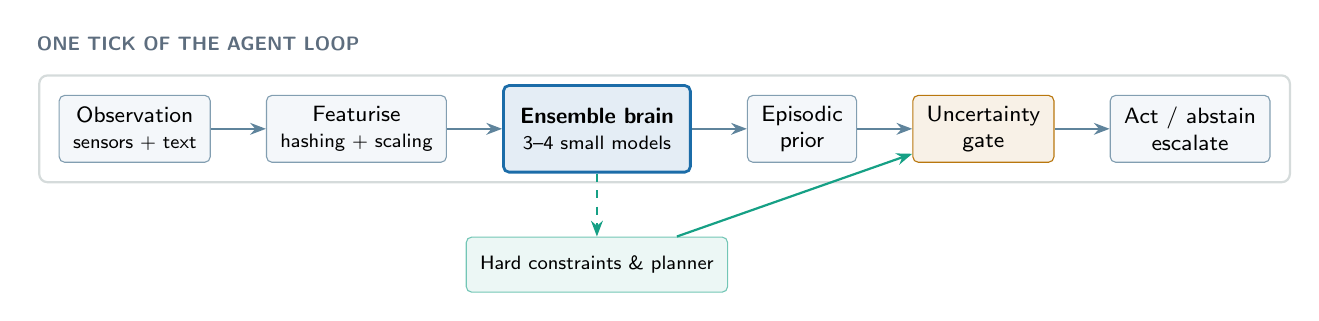
\begin{tikzpicture}[
  font=\sffamily\footnotesize,
  box/.style={draw=conclaveblue!55, fill=conclavebg, rounded corners=2pt,
              minimum height=8.5mm, inner xsep=5pt, align=center},
  core/.style={draw=conclavelight, fill=conclavelight!12, line width=1pt,
               rounded corners=2pt, minimum height=11mm, inner xsep=6pt,
               align=center},
  gate/.style={draw=conclaveamber, fill=conclaveamber!10, rounded corners=2pt,
               minimum height=8.5mm, inner xsep=5pt, align=center},
  ar/.style={-{Stealth[length=2mm]}, conclaveblue!70, line width=0.8pt}]

\node[box] (obs)  {Observation\\{\scriptsize sensors + text}};
\node[box, right=7mm of obs] (feat) {Featurise\\{\scriptsize hashing + scaling}};
\node[core, right=7mm of feat] (brain) {\textbf{Ensemble brain}\\{\scriptsize 3--4 small models}};
\node[box, right=7mm of brain] (mem) {Episodic\\prior};
\node[gate, right=7mm of mem] (gt) {Uncertainty\\gate};
\node[box, right=7mm of gt] (act) {Act / abstain\\escalate};

\draw[ar] (obs)--(feat); \draw[ar] (feat)--(brain); \draw[ar] (brain)--(mem);
\draw[ar] (mem)--(gt);   \draw[ar] (gt)--(act);

\node[draw=conclaveteal!60, fill=conclaveteal!8, rounded corners=2pt,
      below=8mm of brain, minimum height=7mm, inner xsep=5pt,
      align=center, font=\sffamily\scriptsize] (con)
      {Hard constraints \& planner};
\draw[ar, conclaveteal] (con) -- (gt);
\draw[ar, conclaveteal, dashed] (brain) -- (con);

\begin{scope}[on background layer]
  \node[fit=(obs)(act), draw=conclaverule, line width=0.8pt, rounded corners=3pt,
        inner sep=7pt] {};
\end{scope}
\node[anchor=west, font=\sffamily\scriptsize\bfseries, color=conclavegrey]
      at ([yshift=6.5mm,xshift=-4mm]obs.north west) {ONE TICK OF THE AGENT LOOP};
\end{tikzpicture}
\end{center}

\subsection{The seven objects you will actually touch}

\begin{center}
\renewcommand{\arraystretch}{1.28}
\begin{tabular}{@{}>{\raggedright\arraybackslash}p{3.4cm}
                 >{\raggedright\arraybackslash}p{7.0cm}
                 >{\raggedright\arraybackslash}p{5.1cm}@{}}
\toprule
\rowcolor{conclavebg}
{\sffamily\bfseries\color{conclaveblue}Object} &
{\sffamily\bfseries\color{conclaveblue}What it is} &
{\sffamily\bfseries\color{conclaveblue}Lives in} \\
\midrule
\code{Observation}   & One reading of the world: numeric features plus optional text & \file{conclave/core/types.py} \\
\code{FusedFeaturizer} & Turns observations into vectors under a fixed memory budget & \file{conclave/brain/featurize.py} \\
\code{EnsembleBrain} & The committee. Replaces the LLM & \file{conclave/brain/ensemble.py} \\
\code{UncertaintyGate} & Converts disagreement into act / gather / abstain / escalate & \file{conclave/brain/uncertainty.py} \\
\code{ToolRegistry}  & Your capabilities, with typed schemas & \file{conclave/core/registry.py} \\
\code{Agent}         & The loop that ties it together & \file{conclave/core/agent.py} \\
\code{ToolRouter}    & Picks a tool by ranking, not classifying & \file{conclave/brain/router.py} \\
\bottomrule
\end{tabular}
\end{center}

\begin{keybox}[The one idea worth carrying through this document]
A single model gives you a prediction and a confidence number. A \emph{committee}
gives you something a single model cannot: the \textbf{spread of opinion}
between members. CONCLAVE treats that spread as a first-class control signal ---
it is the difference between ``this is a hard call'' and ``I have no idea'',
and those two situations warrant different behaviour. Section~\ref{sec:math}
derives it properly.
\end{keybox}

\subsection{If you have twenty minutes}

\begin{enumerate}[leftmargin=*,itemsep=3pt]
  \item \S\ref{sec:windows} --- set up the virtual environment, run \code{pytest}.
        Expect \textbf{14 passed}.
  \item Run \code{python demo.py episode} and watch the \code{net} column.
        Long stretches say \code{DOWN} and the agent keeps working. That is the
        entire thesis of the project, visible in one column.
  \item Run \code{python demo.py uncertainty} to see the committee split apart
        as you break its sensors.
\end{enumerate}

Everything else in this guide is depth on those three things.

% ======================================================================
\section{Running it on Windows with VS Code}\label{sec:windows}
% ======================================================================

Nothing here is exotic. If you have set up a virtual environment for a Flask
project you already know this workflow; the only unusual part is that a couple
of the experiments spend a few minutes on CPU.

\subsection{Prerequisites}

\begin{center}
\renewcommand{\arraystretch}{1.25}
\begin{tabular}{@{}>{\raggedright\arraybackslash}p{3.6cm}
                 >{\raggedright\arraybackslash}p{4.0cm}
                 >{\raggedright\arraybackslash}p{7.6cm}@{}}
\toprule
\rowcolor{conclavebg}
{\sffamily\bfseries\color{conclaveblue}Thing} &
{\sffamily\bfseries\color{conclaveblue}Version} &
{\sffamily\bfseries\color{conclaveblue}Why} \\
\midrule
Python & \textbf{3.10 -- 3.12} & 3.13 still misses \code{lightgbm} wheels on some Windows builds \\
VS Code & any current & \\
Python extension & \code{ms-python.python} & brings \code{debugpy} and the Testing panel \\
Disk & $\approx$\,700\,MB & mostly \code{scikit-learn} and \code{lightgbm} wheels \\
Network & first install only & the framework never touches the network at runtime \\
\bottomrule
\end{tabular}
\end{center}

\noindent There is deliberately no CUDA, no GPU, and no API key anywhere in
this list.

\subsection{One-time setup}

Open the \file{conclave} folder in VS Code --- \textbf{File\,$\rightarrow$\,Open
Folder}, and pick the folder that \emph{contains} \file{pyproject.toml}, not its
parent. This matters: pointing VS Code at the parent is the single most common
reason \code{pytest} later collects zero tests.

Then open the integrated terminal with \key{Ctrl} + \key{`}:

\begin{codebox}[PowerShell --- one time]
\begin{lstlisting}[style=shell]
py -3.12 -m venv .venv
.\.venv\Scripts\Activate.ps1

python -m pip install --upgrade pip
pip install -e ".[boost,experiments,dev]"
\end{lstlisting}
\end{codebox}

\noindent Your prompt should now start with \code{(.venv)}.

\begin{warnbox}[If PowerShell refuses to run the activation script]
Windows blocks unsigned scripts by default. Unblock it for this terminal only:
\begin{lstlisting}[style=shell]
Set-ExecutionPolicy -Scope Process -ExecutionPolicy Bypass
\end{lstlisting}
\code{-Scope Process} means the change dies with the terminal window, which is
exactly what you want --- do not use \code{-Scope CurrentUser} for this.
\end{warnbox}

\subsubsection{What the three extras install}

\code{pip install -e ".[boost,experiments,dev]"} pulls three optional groups on
top of the core dependencies:

\begin{center}
\renewcommand{\arraystretch}{1.2}
\begin{tabular}{@{}>{\raggedright\arraybackslash}p{2.4cm}
                 >{\raggedright\arraybackslash}p{5.6cm}
                 >{\raggedright\arraybackslash}p{7.2cm}@{}}
\toprule
\rowcolor{conclavebg}
{\sffamily\bfseries\color{conclaveblue}Extra} &
{\sffamily\bfseries\color{conclaveblue}Packages} &
{\sffamily\bfseries\color{conclaveblue}Needed for} \\
\midrule
(core) & numpy, scipy, scikit-learn, joblib, psutil & the framework itself \\
\code{boost} & lightgbm, xgboost & the gradient-boosted committee member \\
\code{experiments} & pandas, pyarrow, matplotlib & running \file{experiments/} and drawing figures \\
\code{dev} & pytest & the test suite \\
\bottomrule
\end{tabular}
\end{center}

\begin{okbox}[LightGBM is optional by design]
If \code{lightgbm} will not install, the framework does not break. \code{ToolRouter}
falls back to scikit-learn's \code{HistGradientBoostingClassifier}, which costs
about half a point of routing accuracy. You can verify which one you got:
\begin{lstlisting}[style=py]
from conclave.brain.router import ToolRouter
print(list(ToolRouter()._default_members()))   # ['lgbm', ...] or ['hgb', ...]
\end{lstlisting}
\end{okbox}

\subsection{Point VS Code at the interpreter}

Press \key{Ctrl}+\key{Shift}+\key{P} $\rightarrow$ \textbf{Python: Select
Interpreter} $\rightarrow$ choose the one under \file{.venv}.

The repository ships a \file{.vscode/settings.json} that already sets this,
enables pytest, and hides \file{\_\_pycache\_\_} from the explorer, so in most
cases it happens by itself:

\begin{codebox}[.vscode/settings.json --- the parts that matter]
\begin{lstlisting}[style=shell]
"python.defaultInterpreterPath": "${workspaceFolder}/.venv/Scripts/python.exe",
"python.testing.pytestEnabled": true,
"python.testing.pytestArgs": ["tests"],
"python.analysis.extraPaths": ["${workspaceFolder}"]
\end{lstlisting}
\end{codebox}

\subsection{Check it works}

\begin{codebox}[PowerShell]
\begin{lstlisting}[style=shell]
pytest -q
\end{lstlisting}
\end{codebox}

\begin{okbox}[Expected]
\textbf{14 passed} in roughly six seconds. Four \code{ConvergenceWarning}s from
\code{SGDClassifier} are normal --- that member is deliberately capped at 25
iterations because it is a committee member, not a soloist.
\end{okbox}

\noindent The 14 tests are two distinct groups, and the distinction is worth
understanding:

\begin{center}
\renewcommand{\arraystretch}{1.25}
\begin{tabular}{@{}>{\raggedright\arraybackslash}p{4.3cm}
                 >{\raggedright\arraybackslash}p{10.9cm}@{}}
\toprule
\rowcolor{conclavebg}
{\sffamily\bfseries\color{conclaveblue}File} &
{\sffamily\bfseries\color{conclaveblue}What it protects} \\
\midrule
\file{tests/test\_smoke.py} & The framework: uncertainty maths, planner, tool
registry, memory, a full agent episode, constraint escalation. Nine tests. \\
\file{tests/test\_paper\_claims.py} & Every number quoted in the paper, checked
against \file{results/*.json}. Five tests. \\
\bottomrule
\end{tabular}
\end{center}

\begin{keybox}[Why the second group exists]
\file{test\_paper\_claims.py} fails \emph{on purpose} if you re-run an experiment
and a number moves. That is not a broken test --- it is the mechanism that stops
the paper and the code drifting apart. When it fails, look at the diff and
decide which one is wrong before you touch either.
\end{keybox}

VS Code's Testing panel (the conical-flask icon in the sidebar) picks these up
automatically and lets you run them one at a time.

\subsection{The debugger, which is where the real understanding happens}

The repository ships eight launch configurations in \file{.vscode/launch.json}.
Press \key{F5} and pick one from the dropdown. The most useful by a wide margin:

\begin{center}
\renewcommand{\arraystretch}{1.25}
\begin{tabular}{@{}>{\raggedright\arraybackslash}p{6.2cm}
                 >{\raggedright\arraybackslash}p{9.0cm}@{}}
\toprule
\rowcolor{conclavebg}
{\sffamily\bfseries\color{conclaveblue}Configuration} &
{\sffamily\bfseries\color{conclaveblue}What it does} \\
\midrule
Demo: watch an episode & The agent decides tick by tick with the network failing \\
Demo: tool routing (interactive) & Type a request, watch it score every tool \\
Exp 3: connectivity loss & The headline experiment, about three minutes \\
\textbf{Debug: break inside Agent.decide} & Same as the episode demo but with
\code{justMyCode: false}, so you can step into scikit-learn \\
\bottomrule
\end{tabular}
\end{center}

\begin{keybox}[The single most useful breakpoint in the project]
Open \file{conclave/core/agent.py}, find \code{Agent.decide}, and put a breakpoint
on the line
\begin{lstlisting}[style=py]
outcome = self.gate(rep.stats)
\end{lstlisting}
Launch \textbf{Debug: break inside Agent.decide}. When it stops, inspect
\code{rep} in the Variables pane. You get \code{rep.member\_probs} --- what each
committee member believed --- and \code{rep.stats}, the full uncertainty
decomposition for that one decision. Everything in \S\ref{sec:math} is visible
there as concrete numbers.
\end{keybox}

\subsection{Reproducing the paper}

\begin{codebox}[PowerShell --- times are for a modest laptop CPU]
\begin{lstlisting}[style=shell]
python experiments/exp3_sequential.py    # ~3 min, no data needed
python experiments/exp5_uncertainty.py   # ~4 min, no data needed
python experiments/exp4_edge.py          # ~1 min, no data needed
python experiments/exp1_tool_routing.py  # ~2 min, needs data/bfcl
python experiments/exp2_humaid.py 12 14  # ~4 min, needs data/humaid
python experiments/make_figures.py       # redraws paper/figures/

python scripts/run_all.py                # or all of the above
\end{lstlisting}
\end{codebox}

\noindent \file{data/} is already in the repository (19\,MB), so every one of
these works offline right now. To re-fetch it: \code{python scripts/fetch\_data.py}.

Each experiment writes a JSON artefact to \file{results/} recording platform,
seed and git commit, so any number can be traced back to the run that produced it.

\begin{warnbox}[One genuine Windows difference]
\file{exp4\_edge.py} enforces a RAM ceiling using \code{RLIMIT\_AS}, which is
POSIX-only. On Windows the code detects this, prints a notice, and reports
thread caps alone --- the memory ceiling becomes advisory rather than enforced.

Everything else is identical across platforms. But do not report an
\emph{enforced} memory ceiling in a paper table from a Windows run, because on
Windows it was not enforced. \S\ref{sec:pi} shows how to get a genuinely
enforced ceiling using containers.
\end{warnbox}

\subsection{When something breaks}

\begin{center}
\renewcommand{\arraystretch}{1.3}
\begin{tabular}{@{}>{\raggedright\arraybackslash}p{5.6cm}
                 >{\raggedright\arraybackslash}p{9.6cm}@{}}
\toprule
\rowcolor{conclavebg}
{\sffamily\bfseries\color{conclaveblue}Symptom} &
{\sffamily\bfseries\color{conclaveblue}Cause and fix} \\
\midrule
\code{ModuleNotFoundError: conclave} & The venv is not active, or you skipped
\code{pip install -e .}. Check for \code{(.venv)} in the prompt. \\
\code{lightgbm} fails to install & You are on Python 3.13. Use 3.12, or accept
the automatic \code{HistGradientBoosting} fallback. \\
\code{pytest} collects 0 tests & VS Code has the parent folder open. Reopen the
\file{conclave} folder itself. \\
Activation script blocked & \code{Set-ExecutionPolicy -Scope Process -ExecutionPolicy Bypass} \\
Experiments feel slow & Expected. \code{exp3} runs 3{,}600 episodes and trains a
committee for each configuration. \\
\code{test\_paper\_claims} fails & You re-ran an experiment and a number moved.
The test is doing its job --- inspect the diff. \\
\bottomrule
\end{tabular}
\end{center}

% ======================================================================
\section{Using the framework}\label{sec:framework}
% ======================================================================

This section builds a complete agent from nothing. The running example is a
solar-powered borehole pump serving a village: it has a tank-level sensor, a
turbidity probe, a battery monitor and a flow meter, plus a text field where a
caretaker types what they see. There is no reliable network. The full file is
\file{examples/pump\_station.py} --- run it with
\code{python examples/pump\_station.py}.

\begin{keybox}[The shape of every CONCLAVE program]
\textbf{tools} $\rightarrow$ \textbf{training observations} $\rightarrow$
\textbf{featuriser} $\rightarrow$ \textbf{brain} $\rightarrow$
\textbf{gate + constraints} $\rightarrow$ \textbf{agent}.\\[2mm]
Six steps, in that order, always. The rest is detail.
\end{keybox}

\subsection{Step 1 --- declare what the agent can do}

A tool is a Python function plus a schema. The \code{@tool} decorator infers the
schema from the type annotations, the way a typed route converter does:

\begin{codebox}[Tools]
\begin{lstlisting}[style=py]
from conclave.tools.base import tool
from conclave import ToolRegistry

@tool(description="Start the borehole pump to refill the tank")
def start_pump(minutes: int = 30) -> str:
    return f"pump running {minutes} min"

@tool(description="Open the chlorine doser to treat the tank", irreversible=True)
def dose_chlorine(ml: int = 50) -> str:
    return f"dosed {ml} ml"

@tool(description="Send an SMS to the maintenance technician")
def call_technician(reason: str = "unknown") -> str:
    return f"SMS sent: {reason}"

registry = ToolRegistry([start_pump, dose_chlorine, call_technician])
\end{lstlisting}
\end{codebox}

\noindent Three arguments to \code{@tool} carry real weight:

\begin{center}
\renewcommand{\arraystretch}{1.25}
\begin{tabular}{@{}>{\raggedright\arraybackslash}p{3.0cm}
                 >{\raggedright\arraybackslash}p{12.2cm}@{}}
\toprule
\rowcolor{conclavebg}
{\sffamily\bfseries\color{conclaveblue}Argument} &
{\sffamily\bfseries\color{conclaveblue}Effect} \\
\midrule
\code{description} & Becomes matchable text for \code{ToolRouter}. Write it the
way a user would describe the need, not the way you named the function. \\
\code{irreversible} & Marks the tool for the constraint layer and lets the
planner exclude it. Dosing chemicals is irreversible; sending an SMS is not. \\
\code{preconditions} / \code{effects} & Predicate lists the planner searches
over. Leave empty if you are not planning. \\
\bottomrule
\end{tabular}
\end{center}

\subsection{Step 2 --- observations}

An \code{Observation} carries numeric features, optional free text, and metadata.
Either modality may be empty; the featuriser handles whichever is present.

\begin{codebox}[Observations]
\begin{lstlisting}[style=py]
from conclave import Observation

Observation(
    features={"tank_level_pct": 11.0, "turbidity_ntu": 1.2,
              "battery_volts": 12.9, "flow_lpm": 0.0},
    text="tank nearly empty this morning",
)
\end{lstlisting}
\end{codebox}

Training data is a list of observations and a matching list of action names.
In the example these are generated synthetically, five scenarios $\times$ 120
samples; in a real deployment they are logged decisions from whoever runs the
station today.

\begin{warnbox}[Two constraints on your training data]
\begin{itemize}[leftmargin=*,itemsep=2pt,topsep=2pt]
  \item \code{EnsembleBrain} needs \textbf{at least two classes}, and enough
        examples per class for its internal cross-validation. A handful of rows
        will raise.
  \item Class names become action names. They must match tool names exactly, or
        \code{Agent} will decide on an action that is not in the registry and
        silently do nothing.
\end{itemize}
\end{warnbox}

\subsection{Step 3 --- featurise under a budget}

\begin{codebox}[Featurisation]
\begin{lstlisting}[style=py]
from conclave.brain.featurize import (BudgetedTextFeaturizer, FusedFeaturizer,
                                   TabularFeaturizer)

fz = FusedFeaturizer(
    text=BudgetedTextFeaturizer(n_word_features=2**12, n_char_features=2**12),
    tabular=TabularFeaturizer(),
).fit(observations)

X = fz.transform(observations)
\end{lstlisting}
\end{codebox}

\begin{keybox}[The feature budget is the deployment knob]
\code{BudgetedTextFeaturizer} uses the hashing trick, so it stores
\textbf{no vocabulary at all} --- its size is fixed when you construct it and
does not grow with your corpus. \code{n\_word\_features} and
\code{n\_char\_features} therefore set the model size directly:
$2^{12}$ gives a 2.6\,MB artefact, $2^{16}$ gives 36\,MB. Table~III of the
paper shows what that costs in accuracy. \S\ref{sec:math} explains why the
hashing trick works and what it costs statistically.
\end{keybox}

\subsection{Step 4 --- the brain}

\begin{codebox}[The committee]
\begin{lstlisting}[style=py]
from conclave import EnsembleBrain

brain = EnsembleBrain().fit(X, labels)

print(list(brain.members_))                        # ['logreg', 'sgd_mh', 'nb']
print(brain.weights_.round(3))                     # [0.333 0.333 0.333]
print(brain.footprint_bytes()["_total"] / 1000)    # 24.2  (KB)
\end{lstlisting}
\end{codebox}

\noindent Twenty-four kilobytes. That is the entire decision-making apparatus
for this agent. \S\ref{sec:models} covers what is inside and how to change it.

\subsection{Step 5 --- the gate and the safety layer}

\begin{codebox}[Uncertainty gate and hard constraints]
\begin{lstlisting}[style=py]
from conclave import UncertaintyGate
from conclave.planning.rules import ConstraintSet, require_confidence

gate = UncertaintyGate(epistemic_max=0.30,   # committee disagreement ceiling
                       aleatoric_max=0.75,   # genuine-ambiguity ceiling
                       confidence_min=0.45,
                       margin_min=0.05,
                       allow_gather=False)   # no cheap extra sensing here

# No statistical model may dose chemicals on a weak majority.
constraints = ConstraintSet([require_confidence(0.80, ["dose_chlorine"])])
\end{lstlisting}
\end{codebox}

\begin{keybox}[The constraint layer sits \emph{above} the learned policy]
A violated constraint does not adjust a probability --- it converts the action
into a recorded \code{ESCALATE}. This is deliberate: no statistical model should
be able to authorise an irreversible act on its own, however confident it
claims to be.
\end{keybox}

\noindent Rather than hand-tuning those four thresholds, you can calibrate them
against a target precision on held-out data:

\begin{codebox}[Calibrating instead of guessing]
\begin{lstlisting}[style=py]
gate = brain.calibrate_gate(X_val, y_val, target_precision=0.90)
print(gate.calibration_)
# {'target_precision': 0.9,
#  'achieved': {'coverage': 0.52, 'precision': 0.906}, ...}
\end{lstlisting}
\end{codebox}

\noindent Read that as: \emph{acting on 52\% of decisions and deferring the rest
buys 90.6\% accuracy on the ones acted upon}. \S\ref{sec:selective} explains the
selective-prediction machinery behind it.

\subsection{Step 6 --- assemble and decide}

\begin{codebox}[The agent]
\begin{lstlisting}[style=py]
from conclave import Agent, EpisodicMemory

agent = Agent(brain=brain, featurizer=fz, registry=registry, gate=gate,
              constraints=constraints, memory=EpisodicMemory(capacity=500))

d = agent.decide(Observation(features=..., text="very cloudy water"))
print(d.action, d.confidence, d.disagreement, d.gate)
\end{lstlisting}
\end{codebox}

\noindent Running the four probe observations from the example file gives:

\begin{codebox}[Actual output of examples/pump\_station.py]
\begin{lstlisting}[style=out]
observation                            action             conf  disag      gate
tank nearly empty this morning         <escalate>         0.65   0.40  escalate
very cloudy water since the storm      dose_chlorine()    1.00   0.00       act
no flow and the battery looks flat     call_technician()  0.78   0.19       act
strange smell from the wellhead ...    <escalate>         0.46   0.35  escalate
\end{lstlisting}
\end{codebox}

All four rows are worth reading carefully, because two of them are the agent
working and two are the agent \emph{knowing it should not act}:

\begin{center}
\renewcommand{\arraystretch}{1.3}
\begin{tabular}{@{}>{\raggedright\arraybackslash}p{4.0cm}
                 >{\raggedright\arraybackslash}p{11.2cm}@{}}
\toprule
\rowcolor{conclavebg}
{\sffamily\bfseries\color{conclaveblue}Row} &
{\sffamily\bfseries\color{conclaveblue}What actually happened} \\
\midrule
cloudy water & Textbook case. Every member agrees (disagreement 0.00), confidence
1.00 clears the 0.80 chlorine constraint, the tool fires. \\
no flow, flat battery & Correct call at 0.78 confidence with mild disagreement.
Note it would \emph{not} have been allowed to dose chlorine at this confidence. \\
strange smell & Nothing like it in training. The committee splits (0.35), the gate
escalates rather than guessing. \textbf{This is the behaviour the whole design
exists to produce.} \\
tank nearly empty & An honest failure. Training said ``tank low overnight draw
down''; the probe says ``nearly empty''. Hashed $n$-grams have no idea those mean
the same thing, so the members split and it escalates. \\
\bottomrule
\end{tabular}
\end{center}

\begin{warnbox}[That last row is a real limitation, not a bug]
CONCLAVE's text features are lexical. They have no compositional semantics, so
paraphrase, negation and synonymy hurt it more than they hurt a transformer.
The paper states this in its limitations; the example reproduces it rather than
hiding it. If your text varies a lot in phrasing, either widen your training
vocabulary or lean harder on the numeric features, which have no such problem.
\end{warnbox}

\subsection{What a \code{Decision} carries}

Every decision is fully auditable --- this matters when an agent is making
consequential calls unsupervised:

\begin{center}
\renewcommand{\arraystretch}{1.22}
\begin{tabular}{@{}>{\raggedright\arraybackslash}p{3.6cm}
                 >{\raggedright\arraybackslash}p{11.6cm}@{}}
\toprule
\rowcolor{conclavebg}
{\sffamily\bfseries\color{conclaveblue}Field} &
{\sffamily\bfseries\color{conclaveblue}Meaning} \\
\midrule
\code{action}        & What it decided: a tool call, or abstain / gather / escalate \\
\code{posterior}     & Probability over every action \\
\code{member\_votes} & What \emph{each} committee member believed, separately \\
\code{confidence}    & Largest posterior probability \\
\code{disagreement}  & Normalised epistemic uncertainty --- the spread of opinion \\
\code{entropy}       & Normalised total uncertainty \\
\code{margin}        & Top-1 minus top-2 probability \\
\code{gate}          & Which branch fired, and therefore why \\
\code{latency\_ms}   & Wall-clock cost of this decision \\
\bottomrule
\end{tabular}
\end{center}

\subsection{Running a sequential environment}

\code{agent.decide()} handles one observation. For a control loop, \code{agent.run()}
drives any environment exposing \code{reset()} and \code{step(action)}:

\begin{codebox}[Episodes]
\begin{lstlisting}[style=py]
from conclave.envs.disaster import DisasterConfig, FloodResponseEnv

episode = agent.run(FloodResponseEnv(DisasterConfig(outage_prob=0.3)),
                    max_steps=40)

print(episode.total_reward, episode.n_escalations)
print(episode.to_dict())          # JSON-serialisable audit trail
\end{lstlisting}
\end{codebox}

\noindent With \code{memory} attached and \code{learn\_online=True} (the default),
successful steps are written back into episodic memory as cases, so the agent
adapts within a deployment without retraining.

\subsection{Tool routing for open vocabularies}

\code{EnsembleBrain} classifies into a \emph{fixed} action set. When tools come
and go at runtime, use \code{ToolRouter} instead: it scores \emph{(request, tool)}
pairs, so a tool registered after training is scored by the same features as
any other.

\begin{codebox}[Routing]
\begin{lstlisting}[style=py]
from conclave.brain.router import ToolRouter

router = ToolRouter(abstain=True, abstain_threshold=0.35).fit(
    queries, candidate_sets, targets)

result = router.route("people stuck on a roof in sector 4, send help",
                      registry.specs())
print(result.tool, result.scores, result.latency_ms)
\end{lstlisting}
\end{codebox}

\noindent \code{result.tool} is \code{None} when nothing scores above the
abstention threshold --- which is the correct answer more often than agent
frameworks like to admit. Try \code{python demo.py route} and give it something
outside its competence; it will show you flat scores rather than a confident
mistake.

% ======================================================================
\section{The machine-learning models inside}\label{sec:models}
% ======================================================================

This is the part that replaces the language model, so it deserves scrutiny.
The short version: CONCLAVE runs a small committee of \emph{deliberately different}
scikit-learn estimators and averages their posteriors. The diversity is not
incidental --- it is the whole mechanism.

\subsection{What is actually in the committee}

\code{EnsembleBrain} picks its default members based on your data. There are
three cases, all decided automatically in \code{conclave/brain/ensemble.py}:

\begin{center}
\renewcommand{\arraystretch}{1.28}
\begin{tabular}{@{}>{\raggedright\arraybackslash}p{3.0cm}
                 >{\raggedright\arraybackslash}p{5.0cm}
                 >{\raggedright\arraybackslash}p{7.2cm}@{}}
\toprule
\rowcolor{conclavebg}
{\sffamily\bfseries\color{conclaveblue}Your data} &
{\sffamily\bfseries\color{conclaveblue}Members} &
{\sffamily\bfseries\color{conclaveblue}Why these} \\
\midrule
Sparse, non-negative \newline {\scriptsize(text only)} &
\code{LogisticRegression}\newline \code{SGDClassifier}\newline \code{ComplementNB} &
Discriminative linear, a differently-regularised linear, and a
\emph{generative} model. Complement NB is the strongest naive-Bayes variant for
imbalanced text. \\
\midrule
Sparse with negatives \newline {\scriptsize(text + scaled sensors)} &
\code{LogisticRegression}\newline \code{SGDClassifier}\newline \code{BernoulliNB} &
Complement NB rejects negative inputs, which appear the moment you standardise
tabular features. Bernoulli NB binarises at zero and accepts either, so the
committee keeps a generative member instead of silently degrading to two linear
models. \\
\midrule
Dense \newline {\scriptsize(sensors only)} &
\code{LogisticRegression}\newline \code{RandomForest}\newline \code{ExtraTrees} &
Linear plus two differently-randomised tree ensembles. Trees dominate on
low-dimensional tabular data. \\
\bottomrule
\end{tabular}
\end{center}

\begin{keybox}[Why heterogeneous rather than one big random forest?]
Because epistemic uncertainty is only meaningful if members can disagree for
\emph{structural} reasons. A random forest's trees share an inductive bias, so
off-distribution they tend to be confidently wrong \emph{together} --- their
disagreement collapses exactly when you need the warning most. Mixing model
families keeps the disagreement signal alive where it matters.
\end{keybox}

\subsection{Two defaults that came from measurement, not taste}

\subsubsection{\code{n\_jobs=1} everywhere}

This looks like a mistake and is not. An agent decides about \emph{one}
observation at a time, over a handful of candidate actions. At that batch size,
constructing a joblib thread pool costs far more than the prediction:

\begin{center}
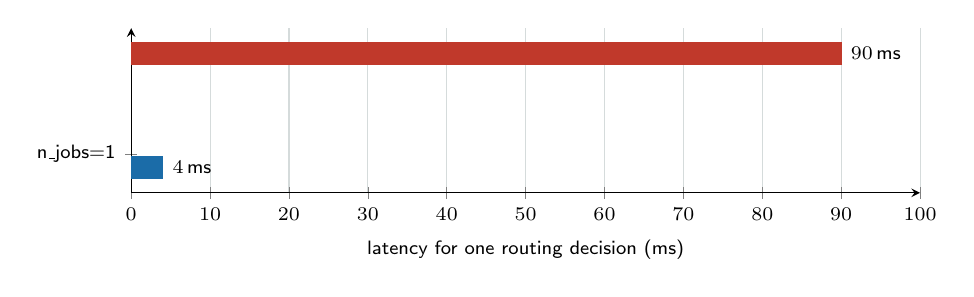
\begin{tikzpicture}
\begin{axis}[
  width=11.6cm, height=4.1cm, xbar, xmin=0, xmax=100,
  bar width=8pt, y=11mm,
  symbolic y coords={n\_jobs=1, n\_jobs=-1}, ytick=data,
  nodes near coords={\sffamily\scriptsize\pgfmathprintnumber\pgfplotspointmeta\,ms},
  nodes near coords align=horizontal,
  xlabel={\sffamily\scriptsize latency for one routing decision (ms)},
  tick label style={font=\sffamily\scriptsize},
  label style={font=\sffamily\scriptsize},
  axis lines=left, enlarge y limits=0.45,
  xmajorgrids, grid style={conclaverule}]
\addplot[fill=conclavelight, draw=conclavelight] coordinates {(4.0,n\_jobs=1)};
\addplot[fill=conclavered, draw=conclavered]     coordinates {(90.0,n\_jobs=-1)};
\end{axis}
\end{tikzpicture}
\end{center}

\noindent Parallelism is a \emph{throughput} optimisation and a \emph{latency}
pessimisation. Edge agents want the latter. If you are ever scoring in bulk
--- offline evaluation, say --- pass \code{n\_jobs=-1} explicitly for that call.

\subsubsection{Shallow, few trees}

Depth-10 forests with 60 estimators lose well under a point of accuracy against
depth-unbounded 200-tree forests, and cut the serialised model roughly
$9\times$. Measured on BFCL routing:

\begin{center}
\renewcommand{\arraystretch}{1.22}
\begin{tabular}{@{}>{\raggedright\arraybackslash}p{6.4cm}rrr@{}}
\toprule
\rowcolor{conclavebg}
{\sffamily\bfseries\color{conclaveblue}Committee} &
{\sffamily\bfseries\color{conclaveblue}Top-1} &
{\sffamily\bfseries\color{conclaveblue}ms/dec.} &
{\sffamily\bfseries\color{conclaveblue}Size} \\
\midrule
RF200 + ET200, \code{n\_jobs=-1}       & 88.6\% & 90.0 & 5\,519\,KB \\
RF200 + ET200, \code{n\_jobs=1}        & 88.6\% & 12.5 & 5\,519\,KB \\
RF100 + ET100, depth 12                & 90.2\% &  7.4 & 1\,332\,KB \\
RF60 + ET60, depth 10                  & 89.2\% &  5.2 &   635\,KB \\
LGBM150 + LogReg                       & 90.2\% &  2.2 &   222\,KB \\
\rowcolor{conclaveteal!10}
\textbf{LGBM200 + RF60d10 + LogReg} \emph{(default)} & \textbf{90.8\%} & \textbf{4.0} & \textbf{631\,KB} \\
\bottomrule
\end{tabular}
\end{center}

\subsection{Swapping the models}

Any scikit-learn-compatible classifier works, provided it exposes
\code{predict\_proba} or \code{decision\_function} (the latter gets softmaxed
automatically). Pass a dict:

\begin{codebox}[A custom committee]
\begin{lstlisting}[style=py]
from sklearn.linear_model import LogisticRegression, RidgeClassifier
from sklearn.ensemble import RandomForestClassifier
from sklearn.neighbors import KNeighborsClassifier
from conclave import EnsembleBrain

brain = EnsembleBrain(
    members={
        "logreg": LogisticRegression(C=2.0, max_iter=500, n_jobs=1),
        "forest": RandomForestClassifier(n_estimators=80, max_depth=10, n_jobs=1),
        "knn":    KNeighborsClassifier(n_neighbors=7),        # instance-based
        "ridge":  RidgeClassifier(alpha=1.0),                 # no predict_proba
    },
    weighting="logloss",     # "uniform" | "accuracy" | "logloss"
    cv=3,
).fit(X, y)

print(brain.weights_.round(3))
print(brain.fit_seconds_)
\end{lstlisting}
\end{codebox}

\begin{center}
\renewcommand{\arraystretch}{1.25}
\begin{tabular}{@{}>{\raggedright\arraybackslash}p{2.6cm}
                 >{\raggedright\arraybackslash}p{12.6cm}@{}}
\toprule
\rowcolor{conclavebg}
{\sffamily\bfseries\color{conclaveblue}\code{weighting}} &
{\sffamily\bfseries\color{conclaveblue}Behaviour} \\
\midrule
\code{"uniform"} & Plain average. The most robust default, and what the paper
uses. Hard to beat when members are comparable. \\
\code{"accuracy"} & Weight by out-of-fold accuracy. Helps when one member is
clearly weaker. \\
\code{"logloss"} & Weight by inverse out-of-fold log loss. Rewards
\emph{calibration}, not just correctness --- usually the better choice when the
posterior itself is being consumed downstream, as it is here by the gate. \\
\bottomrule
\end{tabular}
\end{center}

\begin{warnbox}[Adding members has a cost you can measure]
Every extra member adds its full inference time to \emph{every} decision, and
its serialised bytes to the deployment. Before adding one, check it earns its
place:
\begin{lstlisting}[style=py]
print(brain.footprint_bytes())   # per-member size, and the total
print(brain.fit_seconds_)        # per-member training time
\end{lstlisting}
Three to four members is the sweet spot in every configuration we measured.
\end{warnbox}

\subsection{Choosing a feature budget}

The budget is the single most consequential deployment decision, because the
hashing trick makes model size a constant you choose rather than a function of
your corpus. Measured on HumAID:

\begin{center}
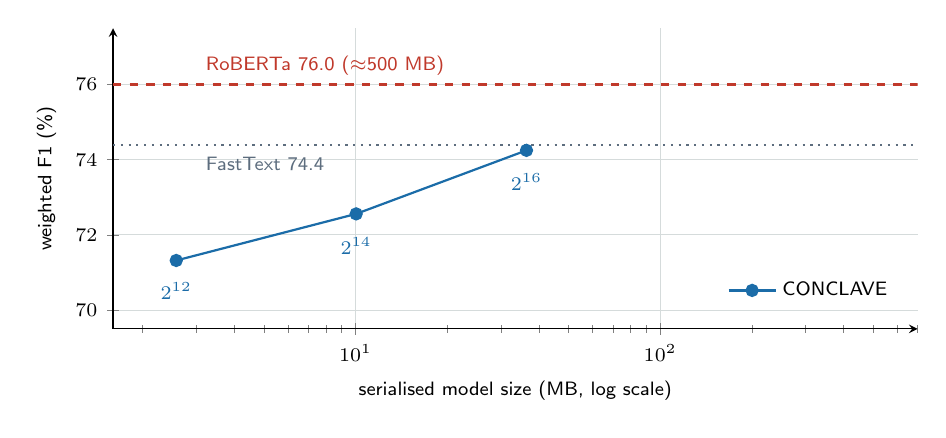
\begin{tikzpicture}
\begin{axis}[
  width=11.8cm, height=5.4cm,
  xlabel={\sffamily\scriptsize serialised model size (MB, log scale)},
  ylabel={\sffamily\scriptsize weighted F1 (\%)},
  xmode=log, xmin=1.6, xmax=700, ymin=69.5, ymax=77.5,
  tick label style={font=\sffamily\scriptsize},
  label style={font=\sffamily\scriptsize},
  legend style={font=\sffamily\scriptsize, draw=none, at={(0.98,0.06)},
                anchor=south east, fill=none},
  axis lines=left, xmajorgrids, ymajorgrids, grid style={conclaverule}]
\addplot[color=conclavelight, mark=*, thick, mark size=2pt]
  coordinates {(2.58,71.32) (10.05,72.56) (36.41,74.25)};
\addlegendentry{CONCLAVE}
\addplot[color=conclavered, dashed, thick, forget plot]
  coordinates {(1.6,76.0) (700,76.0)};
\addplot[color=conclavegrey, dotted, thick, forget plot]
  coordinates {(1.6,74.4) (700,74.4)};
\node[font=\sffamily\scriptsize, color=conclavered, anchor=west] at (axis cs:3,76.5) {RoBERTa 76.0 ($\approx$500 MB)};
\node[font=\sffamily\scriptsize, color=conclavegrey, anchor=west] at (axis cs:3,73.9) {FastText 74.4};
\node[font=\sffamily\scriptsize, color=conclavelight, anchor=north] at (axis cs:2.58,71.0) {$2^{12}$};
\node[font=\sffamily\scriptsize, color=conclavelight, anchor=north] at (axis cs:10.05,72.2) {$2^{14}$};
\node[font=\sffamily\scriptsize, color=conclavelight, anchor=north] at (axis cs:36.41,73.9) {$2^{16}$};
\end{axis}
\end{tikzpicture}
\end{center}

\noindent A practical rule for picking one:

\begin{center}
\renewcommand{\arraystretch}{1.25}
\begin{tabular}{@{}>{\raggedright\arraybackslash}p{2.6cm}
                 >{\raggedright\arraybackslash}p{3.2cm}
                 >{\raggedright\arraybackslash}p{9.4cm}@{}}
\toprule
\rowcolor{conclavebg}
{\sffamily\bfseries\color{conclaveblue}Budget} &
{\sffamily\bfseries\color{conclaveblue}Artefact} &
{\sffamily\bfseries\color{conclaveblue}Use when} \\
\midrule
$2^{12}$ & 2.6\,MB & Microcontroller-class hardware, or text is a minor signal \\
$2^{14}$ & 10\,MB  & Pi Zero / Pi 3 with other things running \\
$2^{16}$ & 36\,MB  & Pi 4 or better; the accuracy plateau starts around here \\
\bottomrule
\end{tabular}
\end{center}

\subsection{Training on your own data}

\begin{codebox}[The whole training path]
\begin{lstlisting}[style=py]
import joblib
from conclave import EnsembleBrain
from conclave.brain.featurize import (BudgetedTextFeaturizer, FusedFeaturizer,
                                   TabularFeaturizer)

fz = FusedFeaturizer(
    text=BudgetedTextFeaturizer(n_word_features=2**14, n_char_features=2**14),
    tabular=TabularFeaturizer(),
).fit(train_obs)

brain = EnsembleBrain(weighting="logloss").fit(fz.transform(train_obs), train_y)
brain.calibrate_gate(fz.transform(val_obs), val_y, target_precision=0.90)

joblib.dump({"fz": fz, "brain": brain, "gate": brain.gate},
            "agent.joblib", compress=3)
\end{lstlisting}
\end{codebox}

\begin{codebox}[Loading on the target device]
\begin{lstlisting}[style=py]
import joblib
from conclave import Agent

bundle = joblib.load("agent.joblib")
agent = Agent(brain=bundle["brain"], featurizer=bundle["fz"],
              registry=registry, gate=bundle["gate"])
\end{lstlisting}
\end{codebox}

\begin{dangerbox}[joblib files are executable code]
\code{joblib.load} unpickles, and unpickling an untrusted file runs arbitrary
code. Only load artefacts you produced yourself or received over a channel you
trust. This is a property of pickle, not of CONCLAVE, but it is your problem the
moment you ship models to field devices.
\end{dangerbox}

\subsection{Where classical models genuinely lose}

Being straight about this is more useful than a sales pitch:

\begin{center}
\renewcommand{\arraystretch}{1.3}
\begin{tabular}{@{}>{\raggedright\arraybackslash}p{4.6cm}
                 >{\raggedright\arraybackslash}p{10.6cm}@{}}
\toprule
\rowcolor{conclavebg}
{\sffamily\bfseries\color{conclaveblue}Weakness} &
{\sffamily\bfseries\color{conclaveblue}What to do about it} \\
\midrule
No compositional semantics & Paraphrase and negation break lexical features.
Widen training vocabulary, or weight numeric features more heavily. \\
Fixed action set (\code{EnsembleBrain}) & Use \code{ToolRouter} when tools change
at runtime --- it ranks pairs, so unseen tools still score. \\
No argument extraction & CONCLAVE selects a tool; it does not fill typed arguments
from free text. Use \code{arg\_builder} on \code{Agent} for rule-based slots. \\
Needs labelled decisions & There is no zero-shot mode. You need examples of the
decision being made, from logs or from an expert controller. \\
\bottomrule
\end{tabular}
\end{center}

% ======================================================================
\section{Deploying and testing for a Raspberry Pi 4}\label{sec:pi}
% ======================================================================

You do not own a Raspberry Pi. That is a normal situation and it does not stop
you from doing most of this properly --- provided you are precise about which
claims survive emulation and which do not. Conflating those two is how resource
claims get rejected in review.

\subsection{Three levels of fidelity}

\begin{center}
\renewcommand{\arraystretch}{1.32}
\begin{tabular}{@{}>{\raggedright\arraybackslash}p{3.3cm}
                 >{\raggedright\arraybackslash}p{5.4cm}
                 >{\raggedright\arraybackslash}p{6.5cm}@{}}
\toprule
\rowcolor{conclavebg}
{\sffamily\bfseries\color{conclaveblue}Level} &
{\sffamily\bfseries\color{conclaveblue}What it is} &
{\sffamily\bfseries\color{conclaveblue}What it can prove} \\
\midrule
\textbf{1. Constrained x86} \newline {\scriptsize what \file{exp4\_edge.py} does} &
Thread caps and a RAM ceiling on your own machine &
Memory footprint, algorithmic behaviour. Latency only as an \emph{x86} number. \\
\midrule
\rowcolor{conclaveteal!7}
\textbf{2. Emulated ARM64} \newline {\scriptsize Docker + QEMU} &
A genuine \code{aarch64} userland: ARM wheels, ARM BLAS, ARM NumPy paths &
That it \emph{installs}, \emph{runs} and \emph{fits} on ARM. Correctness.
\textbf{Not} latency. \\
\midrule
\textbf{3. Real hardware} &
An actual Pi 4, about \$50 &
Everything, including latency and energy \\
\bottomrule
\end{tabular}
\end{center}

\begin{keybox}[What emulation is genuinely for]
Level 2 answers the question that actually blocks a deployment: \emph{does the
software stack exist for this architecture at all?} Whether \code{scipy} has an
ARM wheel is a hard yes/no that emulation answers definitively, and it is a far
more common cause of failed edge deployments than being 3\,ms too slow.
\end{keybox}

\subsection{The finding that will save you a weekend}

Raspberry Pi OS ships in 32-bit (\code{armv7l}) and 64-bit (\code{aarch64})
flavours. For this dependency stack they are not equivalent:

\begin{center}
\renewcommand{\arraystretch}{1.24}
\begin{tabular}{@{}l c c@{}}
\toprule
\rowcolor{conclavebg}
{\sffamily\bfseries\color{conclaveblue}Package} &
{\sffamily\bfseries\color{conclaveblue}PyPI \code{aarch64} (64-bit)} &
{\sffamily\bfseries\color{conclaveblue}PyPI \code{armv7l} (32-bit)} \\
\midrule
numpy        & \textcolor{conclaveteal}{\textbf{wheel}} & \textcolor{conclavered}{\textbf{none}} \\
scipy        & \textcolor{conclaveteal}{\textbf{wheel}} & \textcolor{conclavered}{\textbf{none}} \\
scikit-learn & \textcolor{conclaveteal}{\textbf{wheel}} & \textcolor{conclavered}{\textbf{none}} \\
lightgbm     & \textcolor{conclaveteal}{\textbf{wheel}} & \textcolor{conclavered}{\textbf{none}} \\
psutil       & \textcolor{conclaveteal}{\textbf{wheel}} & \textcolor{conclavered}{\textbf{none}} \\
joblib       & \multicolumn{2}{c}{\textcolor{conclaveteal}{\textbf{pure Python --- fine either way}}} \\
\bottomrule
\end{tabular}
\end{center}

\begin{dangerbox}[Use the 64-bit OS]
On 32-bit Raspberry Pi OS, \code{pip install scipy} means \emph{compiling scipy
on the Pi}. That is hours of build time and it frequently dies of memory
exhaustion on a 1\,GB board.

Two ways out, in order of preference:
\begin{enumerate}[leftmargin=*,itemsep=2pt,topsep=3pt]
  \item \textbf{Install 64-bit Raspberry Pi OS} and use ordinary PyPI wheels.
        The Pi 4 and Pi Zero 2 W are both 64-bit capable. This is the right
        answer.
  \item If you are stuck on 32-bit, use \textbf{piwheels}
        (\code{piwheels.org}), which publishes pre-built \code{armv7l} wheels
        and is already configured as an index on Raspberry Pi OS. It carries
        builds for all four packages above.
\end{enumerate}
\end{dangerbox}

\subsection{Setting up emulated ARM64 on Windows}

\begin{codebox}[PowerShell --- one time]
\begin{lstlisting}[style=shell]
# 1. Docker Desktop with the WSL2 backend must be running.
docker version

# 2. Register the QEMU binfmt handlers so the kernel can execute ARM binaries.
docker run --privileged --rm tonistiigi/binfmt --install arm64

# 3. Confirm arm64 is now a build target.
docker buildx ls
\end{lstlisting}
\end{codebox}

\noindent You should see \code{linux/arm64} listed among the supported
platforms. That single \code{binfmt} step is what makes everything else work:
it teaches the Linux kernel to hand \code{aarch64} executables to QEMU
transparently.

\subsection{Build and run the Pi target}

The repository ships \file{deploy/Dockerfile.pi4} and
\file{deploy/docker-compose.pi4.yml}.

\begin{codebox}[PowerShell --- from the repo root]
\begin{lstlisting}[style=shell]
docker buildx build --platform linux/arm64 `
  -f deploy/Dockerfile.pi4 -t conclave:pi4 --load .

# sanity check: what architecture are we actually on?
docker run --rm --platform linux/arm64 conclave:pi4

# the real check, with a Pi 4's memory ceiling enforced
docker compose -f deploy/docker-compose.pi4.yml run --rm pi4 `
  python deploy/pi_check.py
\end{lstlisting}
\end{codebox}

\noindent Three details in that Dockerfile are deliberate and worth copying if
you write your own:

\begin{center}
\renewcommand{\arraystretch}{1.28}
\begin{tabular}{@{}>{\raggedright\arraybackslash}p{5.4cm}
                 >{\raggedright\arraybackslash}p{9.8cm}@{}}
\toprule
\rowcolor{conclavebg}
{\sffamily\bfseries\color{conclaveblue}Line} &
{\sffamily\bfseries\color{conclaveblue}Why} \\
\midrule
\code{--only-binary=:all:} & Makes a missing ARM wheel fail \emph{loudly} in
seconds instead of silently starting an hour-long source build. This is the
single most useful flag in the file. \\
\code{apt-get install libgomp1} & LightGBM's OpenMP runtime. The
\code{python:slim} images do not ship it, and the resulting \code{ImportError}
is cryptic. \\
\code{OMP\_NUM\_THREADS=1} & Matches the single-decision workload, for the
reason in \S\ref{sec:models}. The compose file raises it to 4 for the Pi 4
profile. \\
\bottomrule
\end{tabular}
\end{center}

\subsection{The compose profiles}

Three boards, with \textbf{real} cgroup limits --- unlike the \code{RLIMIT\_AS}
path in \file{exp4\_edge.py}, which silently does nothing on Windows:

\begin{center}
\renewcommand{\arraystretch}{1.24}
\begin{tabular}{@{}llrrl@{}}
\toprule
\rowcolor{conclavebg}
{\sffamily\bfseries\color{conclaveblue}Service} &
{\sffamily\bfseries\color{conclaveblue}Board} &
{\sffamily\bfseries\color{conclaveblue}RAM} &
{\sffamily\bfseries\color{conclaveblue}CPUs} &
{\sffamily\bfseries\color{conclaveblue}Notes} \\
\midrule
\code{pi4}    & Pi 4 Model B      & 4\,GB   & 4 & the usual target \\
\code{pi3}    & Pi 3B+            & 1\,GB   & 4 & tight but workable \\
\code{zero2w} & Pi Zero 2 W       & 512\,MB & 1 & the hard case \\
\bottomrule
\end{tabular}
\end{center}

\begin{keybox}[\code{memswap\_limit} equal to \code{mem\_limit} disables swap]
Without that, Docker lets the container swap and your ``512\,MB'' test quietly
becomes a 1\,GB test. Setting them equal is what makes the ceiling real. This is
the most commonly botched part of container-based memory testing.
\end{keybox}

\subsection{What \code{pi\_check.py} reports, and why it is split}

\file{deploy/pi\_check.py} trains a small agent, exercises it, and labels every
line \code{[valid]} or invalid, detecting emulation by looking for a real Pi
signature in \file{/proc/cpuinfo} and \file{/proc/device-tree/model}:

\begin{codebox}[One captured run on native 2-core x86 --- your numbers will differ]
\begin{lstlisting}[style=out]
  architecture   : x86_64
  visible cores  : 2
  RAM ceiling    : 3915 MB
  emulated       : no
====================================================================
  [valid]  agent artefact      :    186.2 KB
  [valid]  training accuracy   :     98.19 %
  [valid]  peak RSS            :    194.9 MB
  [valid]  fits RAM ceiling    : YES
  [valid]  training time       :       2.0 s

  [valid (native)]
           median decision     :      2.41 ms
           p99 decision        :      2.92 ms
\end{lstlisting}
\end{codebox}

\noindent Run the same script under the \code{arm64} container and the header
flips to \code{emulated: YES}, the timing block is marked invalid, and the
script tells you so in plain language.

\begin{warnbox}[Latency is noisy; do not quote a single run]
Repeated runs of the same benchmark on the same machine vary by tens of
percent, depending on thermal state and what else is running. Across three runs
of \file{exp4\_edge.py} on the same container the host median moved between
2.4 and 2.8\,ms. If a latency number is going into a paper, report the median
of several independent runs and say how many --- and re-run every experiment
that feeds a table before you submit, because a stale table is the easiest
mistake to make and the hardest to spot.
\end{warnbox}

\subsection{What you may and may not claim}

\begin{center}
\renewcommand{\arraystretch}{1.3}
\begin{tabular}{@{}>{\raggedright\arraybackslash}p{5.0cm}
                 >{\raggedright\arraybackslash}p{10.2cm}@{}}
\toprule
\rowcolor{conclavebg}
{\sffamily\bfseries\color{conclaveblue}Measurement} &
{\sffamily\bfseries\color{conclaveblue}Status under emulation} \\
\midrule
Model / artefact size & \textcolor{conclaveteal}{\textbf{Valid.}} Architecture-independent bytes. \\
Peak RSS & \textcolor{conclaveteal}{\textbf{Valid.}} The cgroup limit is real, and pointer width is genuinely 64-bit ARM. \\
Fits in RAM (yes/no) & \textcolor{conclaveteal}{\textbf{Valid}}, and this is the claim that most often decides a deployment. \\
Correctness / accuracy & \textcolor{conclaveteal}{\textbf{Valid.}} Same wheels, same code paths. \\
Wheel availability & \textcolor{conclaveteal}{\textbf{Valid}}, and only obtainable this way. \\
\midrule
Decision latency & \textcolor{conclavered}{\textbf{Invalid.}} QEMU is typically 5--20$\times$ slower and not uniformly so. \\
Energy per decision & \textcolor{conclavered}{\textbf{Invalid.}} Derived from latency. \\
Throughput & \textcolor{conclavered}{\textbf{Invalid.}} \\
\bottomrule
\end{tabular}
\end{center}

\begin{warnbox}[How to phrase this in the paper]
The paper currently reports estimated on-device latency scaled by a relative
single-core throughput ratio, and labels it an estimate. That is defensible.
What is \emph{not} defensible is presenting a QEMU number as a Pi measurement.
If a reviewer asks for hardware numbers, the honest answer is: ``memory and
correctness were verified on an emulated \code{aarch64} target with enforced
cgroup limits; latency is a stated scaling model, and we have not measured on
silicon.'' Buying a Pi 4 is the cheapest way to close that gap.
\end{warnbox}

\subsection{When you do get real hardware}

\begin{codebox}[On the Pi, over SSH --- 64-bit Raspberry Pi OS]
\begin{lstlisting}[style=shell]
uname -m                       # want: aarch64
sudo apt update && sudo apt install -y python3-venv python3-dev libgomp1

python3 -m venv ~/conclave-env
source ~/conclave-env/bin/activate

git clone https://github.com/<user>/conclave && cd conclave
pip install --only-binary=:all: -e ".[boost]"

python deploy/pi_check.py      # now every line is valid
pytest -q                      # 9 smoke tests; paper-claim tests need results/
\end{lstlisting}
\end{codebox}

\noindent Two practical notes for real hardware:

\begin{itemize}[leftmargin=*,itemsep=3pt]
  \item \textbf{Thermal throttling is real.} A Pi 4 under sustained load drops
        clock speed. Run \code{vcgencmd measure\_temp} alongside your benchmark
        and discard runs above about 80\,\textdegree C, or report that you used
        a heatsink.
  \item \textbf{Pin the governor} before timing anything:
        \code{sudo cpufreq-set -g performance}. Otherwise the first few
        decisions are measured at idle clock and your p99 is meaningless.
\end{itemize}

\subsection{Deploying a trained agent, not the training code}

For a field device you ship the artefact, not the pipeline:

\begin{codebox}[On your laptop]
\begin{lstlisting}[style=py]
import joblib
joblib.dump({"fz": fz, "brain": brain, "gate": brain.gate},
            "agent.joblib", compress=3)     # ~200 KB
\end{lstlisting}
\end{codebox}

\begin{codebox}[On the Pi --- no pandas, no matplotlib, no training data]
\begin{lstlisting}[style=py]
import joblib
from conclave import Agent
from conclave.core.types import Observation

b = joblib.load("agent.joblib")
agent = Agent(brain=b["brain"], featurizer=b["fz"],
              registry=registry, gate=b["gate"])

while True:
    obs = Observation(features=read_sensors(), text=read_radio())
    d = agent.decide(obs)
    log(d.action, d.confidence, d.disagreement, d.gate)
\end{lstlisting}
\end{codebox}

\noindent The runtime dependency set collapses to \code{numpy}, \code{scipy},
\code{scikit-learn}, \code{joblib} --- and \code{lightgbm} only if you use
\code{ToolRouter}. That is roughly 60\,MB of wheels and a 200\,KB agent.

% ======================================================================
\section{The mathematics: where every equation comes from}\label{sec:math}
% ======================================================================

The paper contains one displayed equation and a dozen implicit ones. None of
them are new --- that is the point. CONCLAVE's contribution is the \emph{composition},
so every piece should be traceable to established work. This section states each
one, says where it comes from, shows where it lives in the code, and explains
what it does operationally.

\begin{center}
\renewcommand{\arraystretch}{1.25}
\begin{tabular}{@{}>{\raggedright\arraybackslash}p{4.5cm}
                 >{\raggedright\arraybackslash}p{5.6cm}
                 >{\raggedright\arraybackslash}p{4.9cm}@{}}
\toprule
\rowcolor{conclavebg}
{\sffamily\bfseries\color{conclaveblue}Equation} &
{\sffamily\bfseries\color{conclaveblue}Origin} &
{\sffamily\bfseries\color{conclaveblue}In the code} \\
\midrule
Shannon entropy & Shannon 1948 & \file{brain/uncertainty.py} \\
Soft-voting aggregation & Bayesian model averaging & \file{brain/ensemble.py} \\
Aleatoric/epistemic split & Houlsby et al.\ 2011 (BALD) & \file{brain/uncertainty.py} \\
Margin & Scheffer et al.\ 2001 & \file{brain/uncertainty.py} \\
Vote entropy & Dagan \& Engelson 1995 & \file{brain/uncertainty.py} \\
Risk--coverage, AURC & El-Yaniv \& Wiener 2010 & \file{brain/uncertainty.py} \\
TF--IDF & Sp\"arck Jones 1972 & \file{brain/featurize.py} \\
Hashing trick & Weinberger et al.\ 2009 & \file{brain/featurize.py} \\
Kernel-weighted prior & Nadaraya--Watson & \file{memory/episodic.py} \\
Linear opinion pool & Stone 1961 & \file{core/agent.py} \\
A$^\star$ with admissible $h$ & Hart et al.\ 1968 & \file{planning/planner.py} \\
Paired bootstrap & Efron 1979 & \file{experiments/exp3\_sequential.py} \\
\bottomrule
\end{tabular}
\end{center}

% ----------------------------------------------------------------------
\subsection{Entropy, and why it is normalised}

Shannon entropy of a distribution $p$ over $K$ actions:
\begin{equation}
\mathcal{H}[p] \;=\; -\sum_{k=1}^{K} p_k \log p_k
\eqsrc{Shannon 1948}
\end{equation}

\noindent measured in nats. It is $0$ when $p$ puts all mass on one action, and
maximal when $p$ is uniform, where $\mathcal{H}[\text{uniform}] = \log K$.

Because CONCLAVE compares uncertainty across problems with different numbers of
actions --- five tools here, ten humanitarian categories there --- every
quantity is divided by $\log K$:
\begin{equation}
\tilde{\mathcal{H}}[p] \;=\; \frac{\mathcal{H}[p]}{\log K} \;\in\; [0,1].
\end{equation}

\noindent Without this the same gate threshold would mean different things in
different deployments. In \file{conclave/brain/uncertainty.py} this is the
\code{logk} divisor appearing in every return value.

% ----------------------------------------------------------------------
\subsection{Aggregating the committee}

With $M$ members producing posteriors $p_1,\dots,p_M$ and weights $w_m$ summing
to one, the ensemble posterior is the weighted mean:
\begin{equation}
\bar p \;=\; \sum_{m=1}^{M} w_m\, p_m .
\label{eq:agg}
\end{equation}

\noindent This is the empirical form of Bayesian model averaging: treat the
members as samples from a posterior over models and marginalise. With
\code{weighting="uniform"} all $w_m = 1/M$, which is what the paper uses and is
hard to beat when members are comparable in quality.

\begin{keybox}[Why averaging \emph{probabilities} and not votes]
Averaging hard votes throws away exactly the information the gate needs. Two
committees can both vote 3--1 for the same action while one is unanimous in
spirit ($0.9,0.9,0.9,0.4$) and the other barely decided
($0.51,0.52,0.53,0.49$). Equation~\eqref{eq:agg} keeps that difference;
majority voting destroys it.
\end{keybox}

% ----------------------------------------------------------------------
\subsection{The decomposition --- the one equation in the paper}

This is the equation that earns the committee its place. Total predictive
uncertainty splits into two parts with different operational meanings:

\begin{equation}
\underbrace{\mathcal{H}[\bar p]}_{\text{total}}
\;=\;
\underbrace{\frac{1}{M}\sum_{m=1}^{M} \mathcal{H}[p_m]}_{\textbf{aleatoric}}
\;+\;
\underbrace{\left(\mathcal{H}[\bar p] - \frac{1}{M}\sum_{m=1}^{M}\mathcal{H}[p_m]\right)}_{\textbf{epistemic}}
\label{eq:bald}
\end{equation}

\subsubsection{Where it comes from}

The right-hand bracket is not an arbitrary residual --- it is the \textbf{mutual
information} between the prediction $y$ and the model identity $\theta$:
\begin{equation}
\mathcal{I}(y;\theta \mid x)
= \underbrace{\mathcal{H}\big[\mathbb{E}_{\theta}\, p(y\mid x,\theta)\big]}_{\mathcal{H}[\bar p]}
- \underbrace{\mathbb{E}_{\theta}\big[\mathcal{H}[p(y\mid x,\theta)]\big]}_{\frac1M\sum_m \mathcal{H}[p_m]}
\end{equation}
using the standard identity $\mathcal{I}(y;\theta) = \mathcal{H}(y) - \mathcal{H}(y\mid\theta)$
and approximating the expectation over $\theta$ by the finite committee. This
quantity is the acquisition function from \textbf{Bayesian Active Learning by
Disagreement} (BALD), introduced by Houlsby, Husz\'ar, Ghahramani and Lengyel in
2011 for choosing which point to label next. CONCLAVE repurposes it: instead of
asking \emph{which example should I label}, it asks \emph{should I act at all}.

Using a deliberately diverse ensemble as the stand-in for a posterior over
models follows Lakshminarayanan et al.\ (2017), who showed ensembles give
uncertainty estimates competitive with far more expensive Bayesian methods.

\subsubsection{Why the epistemic term cannot go negative}

Entropy is concave. By Jensen's inequality, for any weights $w_m$,
\begin{equation}
\mathcal{H}\Big[\sum_m w_m p_m\Big] \;\ge\; \sum_m w_m\, \mathcal{H}[p_m],
\end{equation}
so $\mathcal{I} \ge 0$ always, with equality exactly when all members agree.
The code clamps at zero anyway (\code{max(H\_mean - mean\_H, 0.0)}) purely to
absorb floating-point noise.

\begin{okbox}[Verified numerically]
Over 4{,}000 randomly generated committees (2--6 members, 5 actions), the
identity in \eqref{eq:bald} held to $4.4\times10^{-16}$ and the epistemic term
was non-negative in every single case. The check is reproducible; the
degenerate cases below are the ones worth memorising.
\end{okbox}

\subsubsection{What the two terms actually mean}

\begin{center}
\renewcommand{\arraystretch}{1.3}
\begin{tabular}{@{}>{\raggedright\arraybackslash}p{4.2cm}rrr>{\raggedright\arraybackslash}p{5.0cm}@{}}
\toprule
\rowcolor{conclavebg}
{\sffamily\bfseries\color{conclaveblue}Committee state} &
{\sffamily\bfseries\color{conclaveblue}conf} &
{\sffamily\bfseries\color{conclaveblue}alea} &
{\sffamily\bfseries\color{conclaveblue}epis} &
{\sffamily\bfseries\color{conclaveblue}Right response} \\
\midrule
All agree, confident & 0.90 & 0.36 & \textbf{0.00} & Act \\
All agree, all unsure & 0.33 & \textbf{1.00} & 0.00 & Abstain --- more data will not help \\
Members disagree & 0.34 & 0.33 & \textbf{0.67} & Gather or escalate --- out of competence \\
\bottomrule
\end{tabular}
\end{center}

\noindent Rows two and three are the entire argument for the decomposition.
Both have confidence around $0.33$. A single model reporting only ``33\%
confident'' cannot distinguish them --- yet one is a genuinely ambiguous
situation where no amount of extra sensing helps, and the other is the model
being out of its depth. \code{UncertaintyGate} routes them to
\code{ABSTAIN} and \code{GATHER}/\code{ESCALATE} respectively.

\begin{warnbox}[The honest caveat, which is also in the paper]
Measured on CONCLAVE's own benchmarks, the decomposition did \emph{not} beat plain
maximum-posterior confidence at either selective prediction or shift detection
(AUROC 0.955 for the epistemic term versus 0.960 for confidence on novel text).
The theory is clean and the degenerate cases above are real, but on these tasks
the extra machinery did not pay for itself. Equation~\eqref{eq:bald} is
reported because it is what the framework computes, not because the measurement
vindicated it.
\end{warnbox}

% ----------------------------------------------------------------------
\subsection{Margin and vote entropy}

Two cheaper signals the gate also consults. The \textbf{margin} is the gap
between the top two actions,
\begin{equation}
\mathrm{margin}(\bar p) \;=\; \bar p_{(1)} - \bar p_{(2)},
\eqsrc{Scheffer et al.\ 2001}
\end{equation}
where $\bar p_{(i)}$ is the $i$-th largest component. It catches the case where
the top probability is respectable but a rival is right behind it --- a
situation entropy alone smooths over.

\textbf{Vote entropy} discards the probabilities and looks only at which action
each member would pick:
\begin{equation}
V_k = \frac{1}{M}\sum_{m=1}^{M} \mathbf{1}\!\left[\arg\max_j (p_m)_j = k\right],
\qquad
\tilde{\mathcal{H}}[V]
\eqsrc{Dagan \& Engelson 1995}
\end{equation}
This is the original query-by-committee disagreement measure (Seung, Opper and
Sompolinsky, 1992). It is robust to a single badly-calibrated member, because
one member's overconfidence cannot inflate a hard vote.

% ----------------------------------------------------------------------
\subsection{Selective prediction: the risk--coverage curve}\label{sec:selective}

An agent that may decline to act is a \emph{selective classifier}: a pair
$(f,g)$ where $f$ predicts and $g \in \{0,1\}$ decides whether to act.
Its two figures of merit are
\begin{equation}
\mathrm{coverage} = \mathbb{E}[g(x)],
\qquad
\mathrm{selective\ risk} = \frac{\mathbb{E}\big[\ell(f(x),y)\,g(x)\big]}{\mathbb{E}[g(x)]},
\eqsrc{El-Yaniv \& Wiener 2010}
\end{equation}
that is, the error rate \emph{among the decisions actually acted upon}. Sweeping
the gate threshold traces a curve; the area under it (AURC) summarises how well
the uncertainty signal ranks decisions. \code{risk\_coverage\_curve} computes it,
and CONCLAVE reports AURC $=0.946$ on the sequential task.

\code{UncertaintyGate.calibrate} inverts this: given a target precision, it
searches a $24\times24$ grid over $(\text{confidence\_min},
\text{epistemic\_max})$ for the thresholds that \textbf{maximise coverage}
subject to precision-on-accepted $\ge$ target. That is the standard
constrained form of the selective-classification problem, and it is why the
gate's thresholds are calibrated rather than guessed.

% ----------------------------------------------------------------------
\subsection{Text features: TF--IDF and the hashing trick}

\subsubsection{TF--IDF, exactly as scikit-learn computes it}

For term $t$ in document $d$, with $n$ documents and $\mathrm{df}(t)$ containing $t$:
\begin{align}
\mathrm{tf}'(t,d) &= 1 + \log \mathrm{tf}(t,d) && \text{(\code{sublinear\_tf=True})}\\
\mathrm{idf}(t)   &= \log\frac{1+n}{1+\mathrm{df}(t)} + 1 && \text{(\code{smooth\_idf=True})}\\
x_{t,d} &= \mathrm{tf}'(t,d)\cdot \mathrm{idf}(t), \qquad
x_d \leftarrow x_d / \lVert x_d\rVert_2 &&
\eqsrc{Sp\"arck Jones 1972}
\end{align}

\begin{okbox}[Verified against scikit-learn]
Implementing the three lines above by hand reproduces
\code{TfidfVectorizer(sublinear\_tf=True)} to $10^{-12}$. The $+1$ terms are
smoothing, so an unseen term never divides by zero; the sublinear \code{tf}
stops a word repeated twenty times counting twenty times as much.
\end{okbox}

\noindent Because rows are $L_2$-normalised, the dot product between a query
vector and a tool-specification vector \emph{is} their cosine similarity ---
which is precisely feature \#1 of \code{ToolRouter}.

\subsubsection{The hashing trick, and what it costs}

Storing a vocabulary makes the model grow with the corpus. Instead, a hash
function $h : \text{term} \to \{1,\dots,D\}$ maps terms directly to indices:
\begin{equation}
\phi_j(x) \;=\; \sum_{i \,:\, h(i)=j} x_i
\eqsrc{Weinberger et al.\ 2009}
\end{equation}

\noindent The feature space is fixed at $D$ regardless of how much text is seen
--- there is no stored vocabulary at all. This is why \code{n\_word\_features}
sets the artefact size directly, and it is the single most important property
for microcontroller-class deployment.

\begin{warnbox}[CONCLAVE uses the unsigned variant, which is biased]
Weinberger et al.'s analysis relies on a \emph{signed} hash, $\xi(i)\in\{\pm1\}$,
which makes collisions cancel in expectation and preserves inner products
without bias. CONCLAVE sets \code{alternate\_sign=False}, so colliding terms always
add \emph{positively} and similarities are biased slightly upward.

This is a deliberate trade: \code{ComplementNB} requires non-negative inputs,
and keeping a generative member in the committee was judged worth the bias.
With $D = 2^{16}$ collisions are rare enough that it does not show up in the
measurements, but it is a real approximation and worth knowing if you shrink
$D$ aggressively.
\end{warnbox}

% ----------------------------------------------------------------------
\subsection{Episodic memory as a kernel-weighted prior}

Given a query key $z$ and retrieved cases $(z_i, a_i, r_i)$ with similarity
$s_i = \max(0, 1 - d_i)$, the memory produces a prior over actions:
\begin{equation}
\pi_k \;\propto\; \sum_{i \,:\, a_i = k,\; r_i > 0} s_i \, r_i,
\qquad
\pi \leftarrow \pi^{1/T} \big/ \textstyle\sum_k \pi_k^{1/T}
\end{equation}

\noindent This is a Nadaraya--Watson kernel-weighted average with a
truncated-cosine kernel, restricted to cases that were actually rewarded, and
$T$ a temperature that sharpens ($T<1$) or flattens ($T>1$) the result. When no
retrieved case has positive reward it returns the uniform distribution, so
memory never biases a decision it knows nothing about.

The result is combined with the ensemble posterior as a \textbf{linear opinion
pool}:
\begin{equation}
p_{\text{final}} \;=\; (1-\omega)\,\bar p \;+\; \omega\,\pi,
\qquad \omega = \code{memory\_weight} = 0.25
\eqsrc{Stone 1961}
\end{equation}

\noindent A linear pool, unlike a logarithmic one, cannot veto: if either source
assigns an action non-negligible mass it survives. For an agent that must not be
talked out of a correct action by a stale memory, that is the safer choice.

% ----------------------------------------------------------------------
\subsection{The planner, and an honest caveat}

\code{Planner.plan} is A$^\star$ over sets of predicates. With $g(s)$ the cost so
far and $h(s)$ an estimate of the cost remaining, it expands the node minimising
$f(s) = g(s) + h(s)$, and A$^\star$ returns an optimal plan \emph{provided}
$h$ never overestimates --- the admissibility condition of Hart, Nilsson and
Raphael (1968).

CONCLAVE uses the goal-count heuristic:
\begin{equation}
h(s) \;=\; \big|\,G \setminus s\,\big|
\end{equation}
the number of goal predicates not yet satisfied.

\begin{dangerbox}[This heuristic is not admissible in general]
The docstring calls it admissible. That holds only under two assumptions:
\begin{enumerate}[leftmargin=*,itemsep=1pt,topsep=2pt]
  \item every action adds \textbf{at most one} goal predicate, and
  \item every action costs \textbf{at least 1}.
\end{enumerate}
Break either and $h$ can overestimate, and A$^\star$ may return a suboptimal
plan. A concrete case, reproducible in three tools:
\begin{lstlisting}[style=py]
step_a     : effects {a},       cost 0.1
finish_bc  : requires a, effects {b,c}, cost 0.5   # total 0.6  <- optimal
direct     : effects {a,b,c},   cost 1.0
# goal = {a,b,c}   ->   CONCLAVE returns ['direct'], cost 1.0
\end{lstlisting}
At state $\{a\}$ we have $g=0.1$ and $h=|\{b,c\}|=2$, so $f=2.1$ --- but the
true remaining cost is $0.5$. The optimal path is pushed behind the
\code{direct} goal node at $f=1.0$, which is popped first.
\end{dangerbox}

\noindent The shipped disaster tools all have single-predicate effects and unit
costs, so the guarantee holds there. If you add a multi-effect or sub-unit-cost
tool, either accept ``good but not provably optimal'', or restore admissibility
with
\begin{equation}
h(s) \;=\; \big|G \setminus s\big| \cdot \frac{c_{\min}}{e_{\max}},
\end{equation}
where $c_{\min}$ is the cheapest action cost and $e_{\max}$ the most goal
predicates any single action can add. Setting $h \equiv 0$ turns A$^\star$ into
uniform-cost search: always optimal, just slower.

% ----------------------------------------------------------------------
\subsection{The paired bootstrap in the headline experiment}

The connectivity result compares two policies on \emph{the same} episode seeds,
so the comparison is paired. For per-episode differences
$d_i = R_i^{\text{CONCLAVE}} - R_i^{\text{cloud}}$, resample indices with
replacement $B=4000$ times and take the empirical $2.5$th and $97.5$th
percentiles of $\bar d^{*}$:
\begin{equation}
\bar d^{*(b)} = \frac{1}{n}\sum_{i=1}^{n} d_{\,\iota^{(b)}_i},
\qquad
\text{CI}_{95} = \Big[\,Q_{2.5}\big(\bar d^{*}\big),\; Q_{97.5}\big(\bar d^{*}\big)\Big]
\eqsrc{Efron 1979}
\end{equation}

\noindent Pairing matters here: episode difficulty varies enormously (when the
surge arrives, how big it is), and pairing removes that variance instead of
letting it swamp the effect. It is also what lets the paper make its most
important negative claim --- that at zero outage the two are
\emph{indistinguishable}, $\Delta = 0.6$ with CI $[-0.7, 1.9]$ --- which is the
check that the comparison was fair in the first place.

% ----------------------------------------------------------------------
\subsection{Reading list, in dependency order}

\begin{enumerate}[leftmargin=*,itemsep=3pt]
  \item \textbf{Shannon (1948)}, \emph{A Mathematical Theory of Communication} --- entropy.
  \item \textbf{Sp\"arck Jones (1972)} --- inverse document frequency.
  \item \textbf{Hart, Nilsson \& Raphael (1968)} --- A$^\star$ and admissibility.
  \item \textbf{Seung, Opper \& Sompolinsky (1992)}; \textbf{Dagan \& Engelson (1995)} --- query by committee, vote entropy.
  \item \textbf{Breiman (2001)} --- random forests; where ensemble diversity comes from.
  \item \textbf{Rennie et al.\ (2003)} --- complement naive Bayes.
  \item \textbf{Weinberger et al.\ (2009)} --- the hashing trick and its guarantees.
  \item \textbf{El-Yaniv \& Wiener (2010)} --- selective classification.
  \item \textbf{Houlsby et al.\ (2011)} --- BALD; equation~\eqref{eq:bald}. \emph{Start here if you read only one.}
  \item \textbf{Lakshminarayanan et al.\ (2017)} --- ensembles as practical uncertainty.
\end{enumerate}

% ======================================================================
\section*{Appendix --- one-page reference}
\addcontentsline{toc}{section}{Appendix --- one-page reference}
% ======================================================================
\markboth{Appendix}{Appendix}

\subsection*{Commands}

\begin{codebox}[Setup, test, explore]
\begin{lstlisting}[style=shell]
py -3.12 -m venv .venv                        # create
.\.venv\Scripts\Activate.ps1                  # activate (PowerShell)
pip install -e ".[boost,experiments,dev]"     # install

pytest -q                                     # expect 14 passed
python demo.py episode                        # watch the net column
python demo.py uncertainty                    # break the sensors
python examples/pump_station.py               # the worked example

python scripts/run_all.py                     # reproduce the paper
python experiments/make_figures.py            # redraw figures
\end{lstlisting}
\end{codebox}

\begin{codebox}[Emulated Raspberry Pi]
\begin{lstlisting}[style=shell]
docker run --privileged --rm tonistiigi/binfmt --install arm64
docker buildx build --platform linux/arm64 -f deploy/Dockerfile.pi4 -t conclave:pi4 --load .
docker compose -f deploy/docker-compose.pi4.yml run --rm pi4 python deploy/pi_check.py
\end{lstlisting}
\end{codebox}

\subsection*{The six-step program}

\begin{codebox}[Minimal complete agent]
\begin{lstlisting}[style=py]
from conclave import (Agent, EnsembleBrain, EpisodicMemory, Observation,
                   ToolRegistry, UncertaintyGate)
from conclave.brain.featurize import (BudgetedTextFeaturizer, FusedFeaturizer,
                                   TabularFeaturizer)
from conclave.tools.base import tool

@tool(description="What a user would say they need")          # 1. tools
def do_something(arg: int = 1) -> str: ...
registry = ToolRegistry([do_something])

observations, labels = load_my_decision_log()                 # 2. data

fz = FusedFeaturizer(                                         # 3. features
    text=BudgetedTextFeaturizer(n_word_features=2**14,
                                n_char_features=2**14),
    tabular=TabularFeaturizer()).fit(observations)

brain = EnsembleBrain(weighting="logloss").fit(               # 4. brain
    fz.transform(observations), labels)

gate = brain.calibrate_gate(X_val, y_val, target_precision=0.90)   # 5. gate

agent = Agent(brain=brain, featurizer=fz, registry=registry,  # 6. agent
              gate=gate, memory=EpisodicMemory(capacity=2000))

d = agent.decide(Observation(features={...}, text="..."))
print(d.action, d.confidence, d.disagreement, d.gate)
\end{lstlisting}
\end{codebox}

\subsection*{Uncertainty cheat-sheet}

\begin{center}
\renewcommand{\arraystretch}{1.3}
\begin{tabular}{@{}>{\raggedright\arraybackslash}p{3.0cm}
                 >{\raggedright\arraybackslash}p{3.0cm}
                 >{\raggedright\arraybackslash}p{4.0cm}
                 >{\raggedright\arraybackslash}p{4.4cm}@{}}
\toprule
\rowcolor{conclavebg}
{\sffamily\bfseries\color{conclaveblue}Aleatoric} &
{\sffamily\bfseries\color{conclaveblue}Epistemic} &
{\sffamily\bfseries\color{conclaveblue}Meaning} &
{\sffamily\bfseries\color{conclaveblue}Gate fires} \\
\midrule
low  & low  & Clear-cut & \code{ACT} \\
high & low  & Genuinely ambiguous; more data will not help & \code{ABSTAIN} \\
low  & high & Members disagree; out of competence & \code{GATHER} / \code{ESCALATE} \\
high & high & Hard \emph{and} unfamiliar & \code{ESCALATE} \\
\bottomrule
\end{tabular}
\end{center}

\subsection*{Numbers worth remembering}

\begin{center}
\renewcommand{\arraystretch}{1.24}
\begin{tabular}{@{}>{\raggedright\arraybackslash}p{7.4cm}
                 >{\raggedright\arraybackslash}p{7.6cm}@{}}
\toprule
\rowcolor{conclavebg}
{\sffamily\bfseries\color{conclaveblue}Quantity} &
{\sffamily\bfseries\color{conclaveblue}Value} \\
\midrule
Tool routing, BFCL \code{live\_multiple}   & 90.8\% top-1, 4.0\,ms, 631\,KB \\
Routing on tools unseen in training        & 78.9\% (lexical baseline 56.7\%) \\
Abstention (irrelevance detection)         & 84.3\% accuracy, 0.921 AUC \\
HumAID triage, $2^{16}$ features           & 0.743 weighted F1 vs RoBERTa 0.760 \\
Disaster agent artefact                    & 232\,KB \\
Decision latency (2-core x86)              & $\approx$\,2.5--2.8\,ms median \\
Return at 73\% offline                     & CONCLAVE $+33.5$ vs cloud oracle $-127.3$ \\
Selective prediction                       & 96.3\% at full coverage $\to$ 100\% at 50\% \\
Shift detection, novel text                & AUROC 0.955 \\
\bottomrule
\end{tabular}
\end{center}

\subsection*{Things that are true and inconvenient}

\begin{enumerate}[leftmargin=*,itemsep=3pt]
  \item Text features are lexical. Paraphrase and negation hurt more than they
        hurt a transformer.
  \item The aleatoric/epistemic split did not beat plain confidence on these
        benchmarks.
  \item Uncertainty-triggered human oversight lost to \emph{random} oversight in
        the sequential task.
  \item Peak RSS is $\approx$\,200\,MB, dominated by the Python runtime; the
        agent itself is 232\,KB.
  \item The planner heuristic is not admissible for multi-effect or
        sub-unit-cost tools.
  \item On-device latency is a scaling model, not a measurement. No Raspberry Pi
        was harmed in the making of this paper --- because none was used.
\end{enumerate}

\vspace{4mm}
\begin{center}

\begin{tikzpicture}
\draw[conclaverule,line width=0.8pt] (0,0) -- (\textwidth,0);
\node[anchor=north, font=\sffamily\footnotesize\color{conclavegrey},
      text width=\textwidth, align=center] at (0.5\textwidth,-2mm)
     {CONCLAVE 0.1.0 \, \textbullet \, Apache-2.0 \, \textbullet \,
      companion to \emph{Agentic AI Without a Language Model}};
\end{tikzpicture}
\end{center}


\end{document}
